% !TEX root=../index.tex

\chapter{Haar-Like Features}
\label{chap:features}
    È stato già accenato che, parlando di caratteristiche di un oggetto, ci si riferisce alle sue proprietà elementari \emph{osservabili} e \emph{misurabili}.
    La scelta del tipo di caratteristiche dipende, in primo luogo dalla natura della rappresentazione dell'oggetto stesso, in secondo luogo da ciò che si vuole mettere in risalto.

    Il sistema di rilevamento descritto da Zhu e Wong utilizza le \emph{feature di Haar} per la valutazione delle immagini di profondità.
    L'uso di questo tipo di feature costituisce il primo di molti punti di contatto tra il sistema proposto dai due ricercatori ed il framework di face recognition di Viola e Jones. 

    \section{Wavelet di Haar}
    \label{sec:haar_wavelets}
        Le feature di Haar sono un costrutto derivante dalle \emph{wavelet di Haar}.
        Queste ultime costituiscono il primo tipo di wavelet sviluppato, proposte da Alfréd Haar in \cite{Haar10} nel \citeyear{Haar10}.
        La wavelet madre è una funzione oscillante di lunghezza finita.
        L'equazione \ref{eq:mother_wavelet} descrive la wavelet madre di Haar.

        \begin{equation}
            \label{eq:mother_wavelet}
            \psi(x) = 
            \begin{cases}
                1 & 0 \leq t < 1/2 \\
                -1 & 1/2 \leq t < 1 \\
                0 & \text { altrimenti }
            \end{cases}
        \end{equation}

        Furono sviluppate come un esempio di funzioni ortonormali di base per uno spazio funzionale ed, in quanto tale, con esse è possibile esprimere un qualsiasi segnale limitato.
        Inoltre, sotto particolari ipotesi, costituiscono un sistema di rappresentazione duale all'analisi spettrale di Fourier.
        % @TODO È vero?
        % Hanno anche il vantaggio, rispetto a quest'ultimo, di mantenere l'informazione del tempo (approfondire).

        \begin{figure}[h]
            \centering
            \begin{subfigure}[b]{0.48\textwidth}
            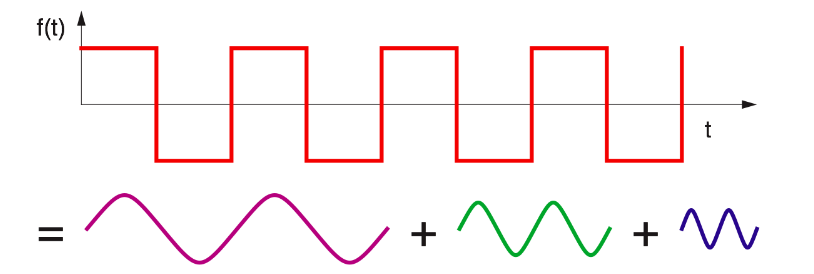
\includegraphics[width=\linewidth]{img/fourier_rapresentation.png}
                \caption{}
                \label{fig:fourier_rapresentation}
            \end{subfigure}
            ~ %add desired spacing between images, e. g. ~, \quad, \qquad, \hfill etc. 
              %(or a blank line to force the subfigure onto a new line)
            \begin{subfigure}[b]{0.48\textwidth}
            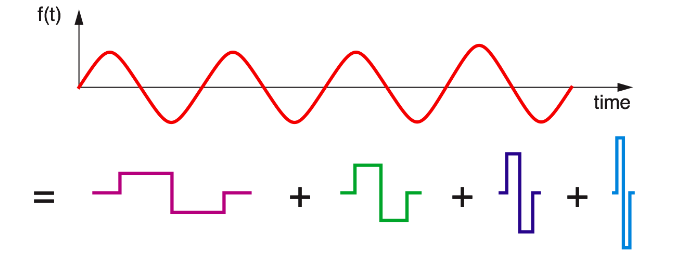
\includegraphics[width=\linewidth]{img/haar_rapresentation.png}
                \caption{}
                \label{fig:wavelet_rapresentation}
            \end{subfigure}
            \caption{Rappresentazione di un segnale con una serie di funzioni armoniche \ref{fig:fourier_rapresentation} e con una serie di wavelet di Haar \ref{fig:wavelet_rapresentation}}
            \label{fig:signal_rapresentation}
        \end{figure}

        Alfrèd Haar propose anche la prima DWT (\emph{Discrete Wavelet Transform}) con la quale, le wavelet che compongono un segnale, vengono campionate discretamente.
        Le applicazioni sono notevoli e ad ampio spettro, prime tra tutte quelle nell'ambito della codica dei segnali e nella compressione dei dati. Per fare un esempio, lo standard di compressione JPEG2000 sfrutta la trasformazione DWT \cite{Jpeg2000} per ottenere risultati qualitativamente migliori rispetto allo standard precedente.

        Una variante della trasformazione DWT con le wavelet di Haar bidimesionali (figura \ref{fig:haar_wavelet}) è stata utilizzata da \citet{Oren97} in un sistema in grado di riconoscere la presenza di pedoni in delle immagini.

        \begin{figure}
            \centering
            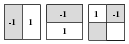
\includegraphics[width=5cm]{img/haar_wavelet.png}
            \caption{Wavelet di Haar bidimensionali utilizzate in \cite{Oren97}.}
            \label{fig:haar_wavelet}
        \end{figure}

        Applicando alle immagini la trasformata DWT in diverse scale, si passa da una rappresentazione dell'immagine in scala dei grigi, ad una rappresentazione in termini di coefficienti delle wavelet di Haar.
        Tali coefficienti denotano le differenze di intensità tra le aree adiacenti dell'immagine e vengono utilizzati per evidenziare analogie strutturali delle immagini che contengono la figura di un pedone.

        \begin{figure}fig      \centering
            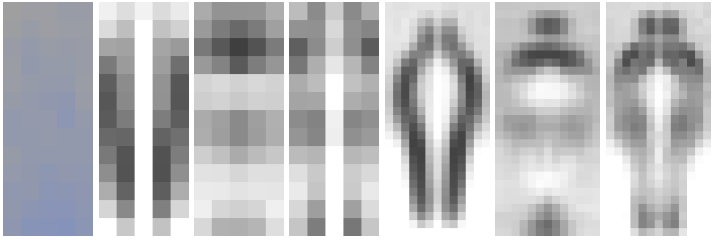
\includegraphics[width=8cm]{img/pedestrian_dwt.png}
            \caption{Coefficienti delle wavelet di trasformate DWT di diverse scale applicate alla stessa immagine. I coefficienti vengono codificati utilizzando la scala dei grigi \cite[Figura 3]{Oren97}.}
            \label{fig:non_standard_dwt}
        \end{figure}

        Nella descrizione di un framework generale per l'object detection, \citet{Papageorgiou98} utilizzano la trasformata DWT a wavelet di Haar bidimensionali non per l'estrazione di un template dell'oggetto espresso in variazioni di intensità, bensì per la selezione delle wavelet più significative al fine del riconoscimento dell'oggetto.

        Una wavelet di Haar bidimensionale di una data dimensione, utilizzata per campionare un'immagine in una posizione specifica mette in evidenza le differenze di intensità dell'immagine nella regione descritta dall'area della wavelet. Tale differenza di intensità costituisce una proprietà osservabile e misurabile dell'immagine che ritrae l'oggetto. Queste sono le \emph{Haar-like feature} o semplicemente \emph{feature di Haar}.

    \section{Definizione} % (fold)
    \label{sec:definizione}
        Le feature di Haar riescono a misurare la quantità e il verso delle variazioni di intensità tra due regioni adiacenti di una immagine.
        La comune rappresentazione grafica mette in evidenza le due regioni colorandone una di bianco e l'altra di nero.
        La somma delle intensità dei pixel della regione bianca, a cui viene sottratta la somma delle intensità della regione nera, fornisce una misura della variazione media di intensità tra le due regioni.

        \begin{equation}
            \label{eq:haar_feature_informal}
            f(Img) = E(Area_{white}) - E(Area_{black})
        \end{equation}

        L'equazione \ref{eq:haar_feature_informal} fornisce una descrizione informale del funzionamento delle feature di Haar. Con $E(Area)$ si intende la somma delle intensità di tutti i pixel che appartengono all'area specificata.

        Al di là di questa iniziale definizione, una feature può essere composta da più di due aree adiacenti, dando luogo alle forme più disparate.
        La libreria \emph{OpenCV} mette a disposizione una grande quantità di feature di forme differenti (figura \ref{fig:opencv_haar_features}).

        Nonostante le forme differenti, il principio resta lo stesso: si hanno sempre due insiemi di aree, quello delle aree chiare ($W$) e quello delle aree scure ($B$).
        Si estende in tal modo la formula per il calcolo del valore della feature:
        \begin{equation}
            \label{eq;haar_feature_general}
            f(Img) = \sum_{Area_i \in W}E(Area_i) - \sum_{Area_j \in B}E(Area_j) 
        \end{equation}

        Il \emph{segno} del valore di una feature identifica il verso della variazione. Se si prende in esame la forma di feature in alto a sinistra della figura \ref{fig:features_type}, un valore positivo denota un'intensità mediamente maggiore nella regione bianca rispetto alla media della regione nera e viceveresa.

        \begin{figure}
            \centering
            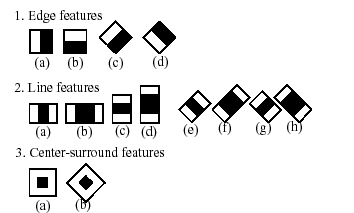
\includegraphics[width=8cm]{img/open_cv_haar_features.png}
            \caption{Set esteso di feature di Haar messe a disposizione dalla libreria \emph{OpenCV}. 
            Le feature inclinate di $45 \degree$ sono state introdotte in \cite{Lienhart02}.}
            \label{fig:opencv_haar_features}
        \end{figure}

        \subsection{Applicazioni} % (fold)
        \label{sub:haar_features_applications}
            Nella framework di riconoscimento dei volti di Viola-Jones, vengono applicate le feature di Haar ad immagini RGB, dopo che queste sono state convertite in scala dei grigi e normalizzate in luminosità.
            Ciò che viene evidenziato sono le differenze di intensità dei pixel tra le regioni della foto.

            A far variare l'intensità di un pixel in una foto concorrono l'illuminazione, il colore e molti altri fattori, alcuni dei quali sono fattori caratteristici del volto, oggetto del riconoscimento, mentre altri sono a tutti gli effetti dei disturbi ambientali che le operazioni di preprocessing mirano ad arginare.

            Esse divengono il mezzo con il quale si può riconoscere un volto umano.
            È stato osservato, ad esempio, che nella foto di un volto, l'area che racchiude entrambi gli occhi e l'inizio del naso è caratterizzato da una particolare variazione di luminosità, misurabile e utilizzabile per descriminare le i volti da i non volti.

            Zhu e Wong le utilizzano su immagini di profondità.
            Vengono considerati solamente quattro tipi di feature, contro i cinque utilizzati da Viola e Jones \ref{fig:features_type}.
            \begin{figure}
                \centering
                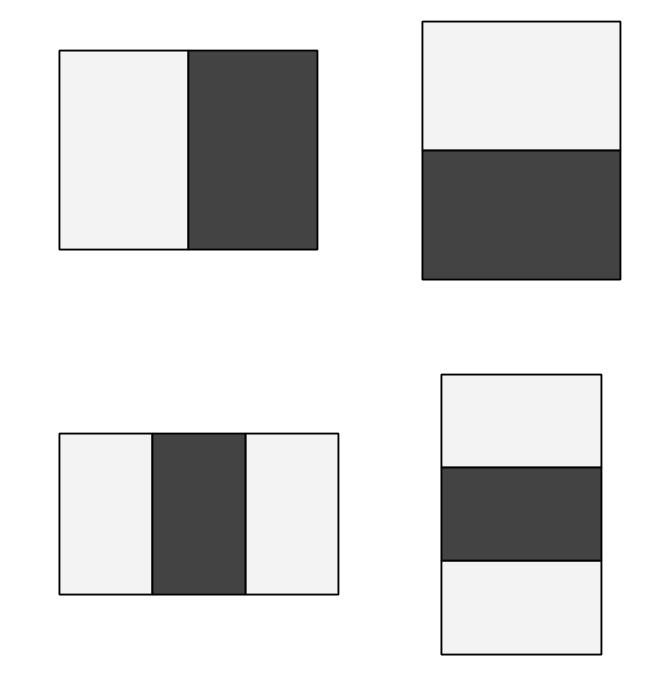
\includegraphics[width=4cm]{img/feature_types.jpg}
                \caption{Tipi di feature di Haar utilizzati in \cite{Zhu13}.}
                \label{fig:features_type}
            \end{figure}

            Nelle immagini di profondità, dove il valore di ogni pixel corrisponde alla distanza in millimetri della superficie dal sensore, applicare le feature di Haar ad un'area dell'immagine equivale a misurare la differenza di quota media rispetto ad un'altra adiacente ad essa.

            Ciò viene utilizzato ai fini del riconoscimento della persona: sarà premura dell'algoritmo di apprendimento selezionare le feature migliori per descrivere la classe delle persone e tali descrizioni si baseranno su osservazioni di differenze di quota, esattamente come la descrizione che, informalmente, è stata data nella sottosezione \ref{sub:hasp}.
        % subsection haar_features_applications (end)

        \subsection{Invarianza ai Ridimensionamenti} % (fold)
        \label{sub:resize_invariance}
            In seguito sarà necessario ridimensionare una feature in modo da coprire un'area più grande, in quanto, dovendo misurare le caratteristiche degli oggetti di interesse, questi ultimi sono variabili in dimensione.
                Il valore calcolato con la feature in questione, tuttavia, non dovrebbe essere troppo sensibile ai ridimensionamenti.

                Al fine di ottenere la massima invarianza ai ridimensionamenti dell'area della feature, il valore di essa viene normalizzato con l'estensione dell'area totale valutata.

                \begin{equation}
                    f'(Img) = \frac
                    {\sum_{Area_i \in W}E(Area_i) - \sum_{Area_j \in B}E(Area_j)}
                    {\sum_{Area_k \in W \cup B}size(Area_k)}
                    \label{eq:haar_scale_invariant}
                \end{equation}

                La tecnica vera e propria utilizzata per ridimensionare una feature verrà presentata nella sezione \ref{sec:detection_tecnique}.
        % subsection resize_invariance (end)

        \subsection{Vantaggi} % (fold)
        \label{sub:haar_feature_vantaggi}
            Il primo indiscutibile vantaggio delle feature di Haar sta nel fatto che la caratterizzazione dell'oggetto viene effettuata sulla base di osservazioni d'insieme su intere aree dell'immagine e non su ossevazioni locali effettuate su singoli pixel.

            Oltre alla grandissima complessità che una valutazione su singoli pixel introdurrebbe, bisogna prendere atto che, con dati soggetti a disturbi e alla presenza di rumore, delle caratteristiche misurate su di essi non sarebbero molto significative.

            L'estrazione dei contorni potrebbe essere più significativo della valutazione sui singoli pixel, ma continuano ad essere caratteristiche abbastanza complesse da calcolare ed ottenere.
            L'estrazione dei contorni, inoltre, è un concetto fortemente legato alle immagini RGB, usarlo con le immagini di profondità è un forzatura.

            Il principale vantaggio delle feature di Haar rispetto ad altri tipi più elaborati di feature resta la loro efficienza computazionale.
            Con una particolare struttura dati di supporto, calcolare il valore di un feature di Haar per un'immagine è un'operazione eseguibile in un tempo costante.
        % subsection haar_feature_vantaggi (end)
    % section definizione (end)
            
    \section{Immagine Integrale}
    \label{sec:integral_image}
        Il calcolo della somma delle intensità di ciascun pixel appartenente ad un'area, necessario al fine di calcolare il valore delle feature di Haar, è un'operazione il cui costo varia all'aumentare della dimensione complessiva dell'area.
        Calcolare tali somme infatti ha complessità computazionale $\Theta(m \cdot n)$ con $m$ ed $n$ dimensione dell'area.

        \begin{figure}
            \centering
            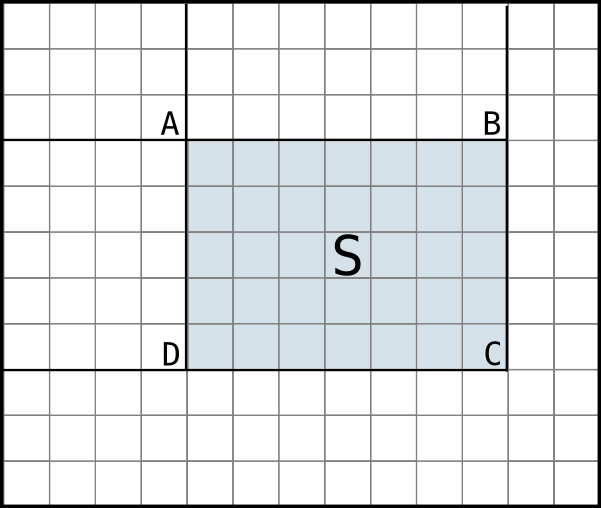
\includegraphics[width=5cm]{img/integral_image_sum.png}
            \caption{}
            \label{fig:integral_image_sum}
        \end{figure}

        La soluzione a tale problema consiste nell'utilizzo dell'\emph{immagine integrale}, altrimenti detta \emph{Summed Area Table}, una struttura dati che mette a permette di calcolare la somma dei pixel di qualsiasi area all'interno di essa in un tempo costante.

        \begin{definition}
            Sia $I$ un'immagine larga $w$ pixel ed alta $h$ pixel. Con la scrittura $I(x, y)$ si identifica il pixel dell'immagine $I$ che si trova alla colonna $x$ e alla riga $y$.
            Si definisce \emph{immagine integrale} (altrimenti detta \emph{Summed Area Table}) una seconda immagine $SAT$ delle stesse dimensioni per cui vale $\forall x \in [1,w], y \in [1,h]$:
            \begin{equation}
                SAT(x, y) = \sum_{i = 1}^{x} \sum_{j = 1}^{y} I(i, j)
            \end{equation}
        \end{definition}

        Calcolare la somma del valore dei pixel contenuti in una regione rettangolare dell'immagine originale, con l'ausilio dell'immagine integrale, è un'operazione velocissima.

        Si consideri la figura \ref{fig:integral_image_sum}: si vuole calcolare la somma del valore dei pixel nella regione $S$ evidenziata. I vertici del rettangolo saranno i punti $A:(x_1,y_1)$, $B:(x_2,y_1)$, $C:(x_2,y_2)$, $D:(x_1, y_2)$, notando che $1 \leq x_1 \leq x_2 \leq w$ e che $1 \leq y_1 \leq y2 \leq h$ \footnote{Nelle immagini raster, si iniziano a contare le colonne e le righe dal punto in alto a sinistra.}.
        Quindi:

        \begin{align*}
            \sum_{i = x_1}^{x_2} \sum_{j = y_1}^{y_2} I(i,j) =
            \sum_{i = 1}^{x_2} \sum_{j = y_1}^{y_2} I(i,j) - \sum_{i = 1}^{x_1} \sum_{j = y_1}^{y_2} I(i,j) = \\
            =
            \left(
            \sum_{i = 1}^{x_2} \sum_{j = 1}^{y_2} I(i,j) -
            \sum_{i = 1}^{x_2} \sum_{j = 1}^{y_1} I(i,j)
            \right)
            -
            \left(
            \sum_{i = 1}^{x_1} \sum_{j = 1}^{y_2} I(i,j) -
            \sum_{i = 1}^{x_1} \sum_{j = 1}^{y_1} I(i,j)
            \right) = \\
            = SAT(C) - SAT(B) - SAT(D) + SAT(A)
        \end{align*}

        Elaborare l'immagine integrale è un'operazione con complessità computazionale $\Theta(w \cdot h)$, cioè il cui costo varia linearmente con la dimensione dell'immagine. Una volta ottenuta però, permette di calcolare qualsiasi somma di pixel in regioni rettangolari con operazioni di complessità $\Theta(1)$.

        L'utilizzo delle immagini integrale è molto vantaggiosa nel momento in cui è necessario calcolare molte feature sulla stessa immagine.
        Volendo essere più espliciti, se la complessità computazionale totale del calcolo di $n$ feature senza l'utilizzo dell'immagine integrale è maggiore di quella per la generazione dell'immagine integrale stessa, allora è vantaggioso utilizzare tale struttura dati.

    \section{Decision Stump}
    \label{sec:decision_stump}
        Una volta misurata una caratteristica relativa ad un oggetto, è necessario trovare un meccanismo, da utilizzare per classificare l'oggetto, che si basi esclusivamente sul valore della misura stessa.        

        \subsection{Definizione di Albero Decisionale}
        Un albero decisionale è un modello predittivo, per il quale, definita una variabile obiettivo, grazie ad una serie di osservazioni e valutazioni di alcune proprietà (o caratteristiche), si giunge a predirne il valore.

        Valgono le seguenti considerazioni:
        \begin{enumerate}
            \item Ogni nodo dell'albero rappresenta una caratteristica osservabile.
            \item Ogni arco dal nodo padre al nodo figlio rappresenta una proprietà, per la caratteristica relativa al nodo padre, che deve essere soddisfatta per percorrere l'arco stesso.
            \item Le foglie dell'albero rappresentano i valori ammissibili per la variabile obiettivo.
            \item Il percorso dalla radice ad una foglia rappresenta la previsione del valore della variabile obiettivo, a fronte delle osservazioni effettuate sulle caratteristiche relative a ciascun nodo attraversato.
        \end{enumerate}

        \subsection{Definizione di Decision Stump}
            Il più semplice albero decisionale è il \emph{decision stump} (letteralmente \emph{ceppo decisionale}), il quale ha profondità unitaria e solamente due foglie.
            Si basa sull'osservazione di una singola caratteristica per le previsioni della variabile obiettivo.

            % Inserire esempio classificazione iris (Fisher) ed immagine

            Alla radice del ceppo decisionale è presente una \emph{funzione di valutazione}\footnote{Il dominio $L$ è costituito da tutte le \emph{formule ben formate}, ovvero da proposizione logiche e dalle relative combinazioni ottenute per mezzo di connettivi logici.} $v:L \rightarrow \{V, F\}$, utilizzata per valutare la caratteristica associata alla radice stessa.
            A seconda del risultato della funzione di valutazione, il percorso terminerà in una o nell'altra foglia.

            Pragmaticamente, intercalando questa iniziale definizione formale nell'attuale contesto applicativo, la radice di ogni ceppo decisionale conterrà un test con cui valutare la feature associata.
            Essendo le feature delle misure a valori reali (quanto meno in questo caso), tutto ciò che bisognerà verificare sarà l'appartenenza della misura ad un preciso range di valori per la selezione del percorso da seguire.

            Si impone un valore di soglia che andrà a partizionare l'immagine della funzione di calcolo della feature: definita la soglia $\theta \in \mathbb{R}$ da associare alla feature $f:Dom(f) \rightarrow Img(f) \in \mathbb{R}$, si partizionerà come segue:
            $$Img(f) = \{f(x)|f(x) < \theta\} \cup \{f(x) | f(x) \geq \theta\}$$

            L'appartenenza della misura ad una o all'altra partizione, decreterà il percorso da seguire verso la foglia.
            In un problema di classificazione binaria, assumendo una classe come classe di oggetti positivi e l'altra come classe di oggetti negativi, associando alla prima il valore simbolico $1$ ed alla seconda $0$, un generico test da porre alla radice del ceppo, può essere della forma \ref{subeq:decision_test_pos} oppure della forma \ref{subeq:decision_test_neg}.

            \begin{equation}
                \label{subeq:decision_test_pos}
                h_1(x) =
                \begin{cases}
                    1 & \text{ se } f(x) > \theta \\
                    0 & \text{ altrimenti }
                \end{cases}
            \end{equation}
            \begin{equation}
                \label{subeq:decision_test_neg}
                h_2(x) = 
                \begin{cases}
                    1 & \text{ se } f(x) < \theta \\
                    0 & \text{ altrimenti }
                \end{cases}
            \end{equation}

            Questi test non fanno altro che discriminare gli oggetti, misurandone una feature, in due classi distinte, a seconda che il valore misurato sia al di sotto o al di sopra del valore di soglia.
            Volendo trovare una descrizione formale unica, si introduce un ulteriore parametro $p \in \{-1,1\}$, detto \emph{polarità}, il cui unico compito è quello di invertire il segno della disequazione, permettendo di fondere le formule \ref{subeq:decision_test_pos} e \ref{subeq:decision_test_neg} in \ref{eq:decision_stump_test}.

            \begin{equation}
                \label{eq:decision_stump_test}
                h(x) = 
                \begin{cases}
                    1 & \text{ se } pf(x) < p\theta \\
                    0 & \text{ altrimenti }
                \end{cases}
            \end{equation}

